\documentclass[11pt,preprint]{aastex}
%\documentstyle[11pt,psfig,aaspp4]{article}
\begin{document}

\def\simlt{\lower.5ex\hbox{$\; \buildrel < \over \sim \;$}}
\def\simgt{\lower.5ex\hbox{$\; \buildrel > \over \sim \;$}}

%{\noindent Astronomy 121 \hfill 2005jan18}

\title {RADIO INTERFEROMETRY AT X BAND \\ \today}

\tableofcontents

The purpose of this lab is, broadly speaking, to learn radio
interferometry---the basis for much of modern radio astronomy. We'll
cover the basic principles, the interferometric fringe, the response to
a point source, and the response to an extended source (which is the
basis of high-angular resolution mapping with interferometry). We will
employ least-squares fitting and Fourier transforms to measure accurate
positions for a few sources and also accurate angular diameters for the
Sun and Moon. And because this is your first foray into observations,
you need to learn about astronomical coordinate systems, topocentric
coordinate systems, converting coordinates with rotation matrices,
systems of civil time, sidereal time. This lab runs for four weeks and
clearly there's a lot of new material!

\section{GOALS}

\begin{itemize}

\item Learn how diffraction theory applies to a real radio
  interferometer. Fringes, their amplitudes and phases. The Fourier
  transform relationship between interferometer response and sky
  brightness. 

\item Learn about all those things observers need to know: time,
  coordinates, conversions.

\item Obtain horizon-to-horizon data on our various astronomical
  sources---point sources, and the Sun and Moon.

\item Learn about linear and nonlinear least-squares fitting and use it
  to tease out accurate source positions.

\item Use least-squares fitting to obtain accurate diameters for the Sun
  and Moon.

\end{itemize}

\section{SCHEDULE}

\begin{enumerate}

\item 6 Feb to 13 Feb: Each {\it person} uses rotation matrices to
calculate when objects of interest are up. Each {\it group} observes the
Sun for a short time to confirm that you see fringes. Each {\it group}
does a horizon-to-horizon observation of a point source, which requires
writing an observing script to run automatically.

Each {\it person} calculates Fourier power spectra of the Sun data and
also the point-source data. She/He calculates the range of expected
local fringe frequencies and compares the observed spectra with these
expectations. Be ready for show and tell!

\item 13 Feb to 20 Feb: Each group observes horizon-to-horizon the Sun
  and, if possible, the Moon with the interferometer.  Each person
  derives accurate declinations for the point-source data using
  least-squares fitting as outlined in \S \ref{declinations}.

\item 20 Feb to 27 Feb: Finish the Moon observations. Each person
  derives accurate angular diameters for the Sun and Moon using
  least-squares fitting as outlined in \S \ref{mun}. 

\item 27 Feb to 6 Mar: Each person finishes all calculations and
writes the lab report, due on 6 Mar.

\end{enumerate}

\section{OUR INTERFEROMETER}

	With our interferometer, which operates at about 11 GHz, our
attention focuses on small sources.  Our interferometer has a relatively
short baseline and the fringe spacing is larger than the size of all
sources (except the Sun and Moon).  So for our interferometer all of
these sources look like ``point sources'', for which all the radiation
appears to come from a single point---just like a star in optical
astronomy.  The output of the interferometer is a sinusoidal-like signal
called the ``fringe''. All of the information resides in the amplitude
and phase of the fringe.

 If you know the baseline, the fringe properties are direct indicators
of the point-source declination.  With our 10-m baseline we can get a
fringe spacing $\sim 10'$, and with a horizon-to-horizon measurement we
can measure the declination 100 times more accurately.  In addition, we
can achieve partial angular resolution on the Sun and Moon and measure
their diameters to a fraction of a percent---this turns out to be more
interesting than it sounds!

We have a {\it multiplying} interferometer: the signals from the
two telescopes are multiplied together. This is equivalent to adding the
signals and then squaring. Actually, it's much better because the
average value of the product is zero, so any detected signal has to come
from the sky instead of the instrument.  So when we look at a source, the
fringe amplitude has no zero offset and the amplitude is directly
proportional to the source flux (if it's a point source). 


\section {CONTINUUM SOURCES}

	For the first part of the lab we will concentrate on measuring
source positions. Our telescopes are small, so there are only a few
sources that are powerful enough for us. The strongest continuum sources
are

$$\vbox{\halign{ \hfil#\hfil\ \ & \hfil#\hfil\ \ & \hfil#\hfil\ \ &    
\hfil#\hfil\ \ & \hfil#\hfil\ \ & \hfil#\hfil\ \ \cr

name & r.a.(1950) & dec(1950) & r.a.(1998) & dec(1998) & $S_{Jy}$ \cr

3C144 (Crab Nebula) & $05^h31^m30^s$ & $21^\circ 58'$
                    & $05^h34^m23^s$ & $22^\circ 00'$ & $\sim 496$ \cr
Orion Nebula        & $05^h32^m44^s$ & $-05^\circ 25'$
                    & $05^h35^m05^s$ & $-05^\circ 23'$ & $\sim 340$ \cr
3C274 (Virgo A)     & $12^h28^m18^s$ & $12^\circ 40'$
                    & $12^h30^m44^s$ & $12^\circ 24'$ & $\sim 34$ \cr
M17                 & $18^h17^m33^s$ & $-16^\circ 12'$
                    & $18^h20^m19^s$ & $-16^\circ 11'$ & $\sim 500$ \cr
3C405 (Cygnus A)    & $19^h57^m45^s$ & $40^\circ 36'$
                    & $19^h59^m24^s$ & $40^\circ 44'$ & $\sim 120$ \cr  
3C461 (Cas A)       & $23^h21^m07^s$ & $58^\circ 34'$
                    & $23^h23^m17^s$ & $58^\circ 50'$ & $\sim 320$ \cr 
SUN                 &   varies       &   varies \cr
MOON                &   varies       &   varies \cr
\cr
}}$$

\noindent You'll need to precess these coordinates to the current
equinox. If you don't, the incorrect r.a.'s will affect your fits. To do
the precession, use the GSFC IDL procedure {\tt precess}. We've supplied the
1998 positions as a guide to whether you are using {\tt precess} correctly.

\subsection{The Point Sources}

	Our goal is to measure their absolute declinations as accurately
as possible.  The positions quoted above are accurate to only about 1
arcminute.  Declinations can be measured on an absolute basis with
interferometry by least-squares fitting the fringe phase to the hour
angle; see {\it Commentary} below.  With our fringe spacing of $\sim
10'$ we might be able to measure declinations to an accuracy $\sim
20''$---maybe better. 

	If possible, we want to measure the difference in right
ascension between the sources.  We can't measure the {\it absolute}
right ascensions because the right ascension coordinate has no
naturally-determined zero point; rather, its zero point is defined
arbitrarily by convention (and it changes with time, too).  In contrast,
declination has a naturally-determined zero point: the equator.  But we
can measure the {\it relative} right ascension of one source with
respect to another with high accuracy.  At least we can do this in
principle; in practice it's harder than measuring only the declinations.

	We'll want {\it each group} to pick a source and obtain a
horizon-to-horizon observation of the fringes. Groups should compare
results to see if you can get the differences in right ascensions (we've
never successfully done this before!). And we'll want {\it each person}
to measure the source's declination by least-squares fitting the
horizon-to-horizon track of fringe phase and amplitude.  Compare your
results with other members of your group.  Help each other out, but {\it
each person should write her/his own software}. 

	There are some considerations in picking sources, and we will
save you some frustration by telling you about them beforehand:
\begin{enumerate}


	\item The fringe frequency depends on $\cos \delta$. This
means that you don't measure $\delta$ directly, but rather $\cos
\delta$. Can you get accurate declinations for sources near $\delta =
0$?

	\item Southern sources are difficult for horizon-to-horizon
tracks because of the presence of the Campanile. 

	\item Our telescope pointing for Northern sources may be
inaccurate, leading to loss of signal/noise. 

	\item Our observing frequency is in the TV satellite band. 
Geostationary TV satellites sit in the southerly skies and generate
strong signals that can enter the dish sidelobes and produce fringes. 

\end{enumerate}

\subsection{The Sun and Moon}

	The Sun and Moon are special cases, for two reasons. First, 
their positions change from day to day---and for the Moon, the change in
just an hour is significant\footnote{Use what you already know to make
an order-of-magnitude estimate of how far the Sun and Moon move in one
day!}.  Second, they are both extended sources, not point sources. This
causes their fringe amplitudes and phases to change with time, in a
manner that depends on their brightness distribution\footnote{These
changes in fringe properties are exactly what's necessary to map the
sources!}; this makes the determination of accurate positions a bit
tricky, but we'll ignore that detail for now.

	You can get the Sun and Moon positions from our IDL procedures
{\tt isun} and {\tt imoon}.  For the Moon, you should be aware that it
is nearby so that you have to correct for your location on the Earth's
surface. The parallax effect is far greater for the Moon than the
Sun---so large that unless you correct for it, the Moon will probably
lie outside the telescope main beam! {\tt imoon} takes care of this
automatically unless you tell it not to\footnote{If you specify the {\tt
geocentric} option, {\tt imoon} gives the lunar position as seen from
the center of the Earth. You {\it don't} want to use this option!}.  A
previous lab TA, Erik Shirokoff (now a Berkeley Physics grad student),
worked very hard to get the moon position, including parallax, really
right; he wrote {\tt imoon}. We think it works. We {\it hope} it works!

	Given these difficulties, why bother with the Sun and Moon?
Because they are {\it bright}. We include them because they provide huge
signals, which is ideal for testing your observing setup and your
reduction software.  In particular, the Sun is so bright that you'll get
a huge signal/noise and you should be able to estimate an accurate
declination in the first few minutes. And if you don't see the Sun, you
{\it know} you're doing something wrong!

\subsection{Some Astrophysics}

Here's a bit of physical information.  M17 (``M'' for Messier) and Orion
are HII regions---places where hot stars have produced warm ($T \sim
10^4$ K) ionized gas, where the electrons flying past the protons get
deflected and produce {\it free-free (bremsstrahlung)} radiation.  The
Sun also emits free-free radiation, just like the HII regions.

The other sources radiate in {\it synchrotron} radiation---relativistic
electrons gyrating in a magnetic field.  For these sources, the source
designation 3CXYZ designate source number XYZ from the third Cambridge
(England) catalog; in the early 1960's, Cambridge radioastronomers
produced the first reliable comprehensive catalog of strong radio
sources in the Northern hemisphere.  The Crab Nebula (also called Taurus
A) is powered by the Crab pulsar, and is a $\sim 1000$ yr-old supernova
remnant in the Galaxy about 1 kpc distant. Cas A is another supernova
remnant, {\it not} powered by a pulsar; rather, the relativistic
electrons are produced behind the fast shock wave produced by the
explosion.  Cas A is $\sim 300$ yr old and about 2.5 kpc distant.  Both
of these supernova remnants are expanding rapidly, as befits their young
ages, and Cas A (in which a pulsar does not constantly replenish the
electrons) is gradually getting dimmer.

In the external galaxies, the ultimate source of the
electrons involves acceleration of electrons near the black hole at the
center; the electrons are then spewed out to extragalactic space in
narrow collimated jets, and produce large ``emission lobes'' at the end
of the jets.  Virgo A is a ``peculiar''
elliptical galaxy about 11 Mpc distant, while Cygnus A is a giant
elliptical galaxy 220 Mpc distant.  Cyg A is a powerful radio
source---it's $10^5$ times further than Cas A and just as bright! The
study of the mechanism by which this enormous power is generated, which
implies enormous energies, has led to the current awareness of and
interest in {\it high-energy astrophysics}.
For information on both types of source and some beautiful
pictures, see chapters 10 and 13 in {\it Galactic and Extragalactic
Radio Astronomy, second edition} (1988, ed.  G.L.  Verschuur and K.I. 
Kellermann). 

	The Moon is a completely different story. Contrary to what you
might expect, at radio wavelengths it {\it doesn't} shine by reflected
sunlight. Rather, its emission is blackbody radiation from its solid
surface. Its surface is heated by sunlight, and at short wavelengths
(but not at long ones) there's a big difference between the temperature
of the sunlit and dark parts of the Lunar surface. You can tell a lot
about its surface properties from the polarization of the radiation and
also from its time variability as the surface heats up from sunlight and
cools off from darkness---just like the Sahara.

\section {MEASURING ACCURATE DECLINATIONS} \label{declinations}

\subsection{General Description}

	We measure declinations from the fringe frequency, which depends
on the baseline orientation, baseline length, declination, and hour
angle (all these go into the {\it projected baseline}. If we observe a
source horizon-to-horizon, the projected baseline changes a lot, and so
does the fringe frequency. We take those data and do a least-squares
fit to derive the most accurate declination from our data.

	{\it FIRST WEEK:} Before doing the weak sources in the Table, do
the Sun for a much shorter time, say an hour. This will give you
confidence that the system works (or so we hope). There should be an
easily-recognizable signal that you can look at visually, think about,
and derive the approximate declination with pencil and paper. Then later
you can write software to do the same, and make sure you get the right
answer.  Also, during this first week, do the horizon-to-horizon track
of one of the sources from the Table.

	Below we'll distill the formulae given in the appendix of the
recommended reference to the nice, straightforward case of an east-west
baseline of length $B$, for which the only nonzero baseline component is
$B_y$. Our interferometer has an east-west baseline, so our distilled
formulae will be applicable to your measurements.  

\subsection{The Details}

	The two interferometer telescopes have different distances from
the source. The difference can range from zero (if the source is
overhead) to nearly the the full baseline (if the source is near the
horizon). This distance difference is tiny compared to the distance to
the source, but it's important! 

	It's convenient to think of the different distances in terms of 
relative path delay in {\it time} units for the two telescopes; we call
this the {\it geometrical} path delay $\tau_g$.  But don't forget! The
signals travel through a lot of electronics before they get multiplied
and the two paths aren't of equal length, so there is an additional
relative delay from the difference in cable length $\tau_c$.  The total
relative delay is the sum of the two,

\begin{equation}
 \tau_{tot} = \tau_g(t) + \tau_c \; . 
\end{equation}


\noindent We explicitly include the fact that $\tau_g$ is a function of
time---it depends on the hour angle. In contrast, $\tau_c$ is
independent of time (unless somebody changes the cable setup\dots).

	We don't know $\tau_c$ (but the least-squares process can tell
us what it is).  However, we do know $\tau_g$ because it's just
geometry---the geometry discussed in the reading.  For the east-west
baseline, we have

\begin{equation}
 \tau_g(t) = \left[{B_y \over c} \cos \delta \right] \sin h \; . 
\end{equation}


	The output of the interferometer is the product of what the two
telescopes see. If they are looking at a monochromatic source then the
voltages for the two telescopes are

\begin{equation}
 E_1(t) = \cos (2 \pi \nu t) 
\end{equation}


\begin{equation}
 E_2(t) = \cos (2 \pi \nu [t + \tau_{tot}]) \; . 
\end{equation}


\noindent and the product is the interferometer fringe output

\begin{equation}
 F(t) = \cos (2 \pi \nu t) \cos (2 \pi \nu [t + \tau_{tot}]) \; . 
\end{equation}


\noindent There's a trigonometric identity that allows us to write this
in terms of the sum and difference of the two
arguments\footnote{$\cos(A) \cos(B)= {1 \over 2}[\cos(A-B) +
\cos(A+B)]$}. The sum term varies rapidly with time and averages to zero;
it's the difference term we want, so if we exclude the sum term (and
forget about the factor $1 \over 2$) we get

\begin{equation}
 F(t) = \cos (2 \pi \nu [\tau_{g}(t) + \tau_c]) \; . 
\end{equation}


	We want to use a least-squares fit to find the values of
quantities that comprise the argument of the cosine.  If you have done
least-squares fitting before (and if you remember anything about it!)
you'll realize that the straightforward least-squares fitting technique
won't work on this type of problem.  We can simplify things for the
fitting process by using another trig identity\footnote{$\cos(A+B) =
\cos(A)\cos(B) - \sin(A)\sin(B)$} and writing this as the
sum of two trig functions

\begin{equation}
 F(t) = \cos(2 \pi \nu \tau_c) \cos \left[2 \pi \nu \left({B_y \over c}
	\cos\delta \right) \sin h\right] - \sin(2 \pi \nu \tau_c) 
	\sin \left[ 2 \pi \nu \left({B_y \over c}\cos\delta \right) \sin h\right] \; .  
\end{equation}


\noindent This may not look simpler! But it is, because for the purposes
of least-squares it involves only a {\it single} variable in the trig
function arguments---the combination of variables $\left({B_y \over c}
\cos\delta \right)$ (we are assuming that we know the right ascension
well enough to get a good value for $h$). 

	To proceed with least-squares, replace $\cos (2 \pi \nu \tau_c)$
and $\sin (2 \pi \nu \tau_c)$ by two ``unknown constants'' $A$ and $B$,
respectively; assume that they are unrelated and solve for them using
the standard least-squares process. Also, it's convenient and intuitive
to make the substitution 

\begin{equation}
\nu \left( {B_y \over c} \cos \delta \right) = \left( {B_y \over \lambda}
\cos \delta \right)
\end{equation}

\noindent which expresses the delay in units of wavelength, and thus the
``number of turns'' or phase. These substitutions give

\begin{equation} \fbox{$
\label{fringeresponse}
 F(t) = A \cos \left[2 \pi \left( {B_y \over \lambda} \cos\delta \right) \sin h\right] 
 - B \sin \left[2 \pi \left( {B_y \over \lambda} \cos\delta \right) \sin h\right] \; . 
$}
\end{equation}

	Let's take a moment and reflect on this complicated-looking
equation, focusing on just the first term (because the second is
identical except it's a sine instead of a cosine). We want to develop
the concept of a {\it local fringe frequency} $f_f$. The argument of the
cosine is a constant $C=\left[2 \pi \left( {B_y \over \lambda}
\cos\delta \right)\right]$ multiplied by $\sin( h)$. Now $h$ is the hour
angle and increases monotonically with time, so we can regard it as
time\footnote{Except that its units are radians. This is no problem: 24
hours is $2\pi$ radians.}. Now $C$ is multiplied not by $h$ itself, but
rather by $\sin( h)$, which is a nonlinear function of time. The product
$C \sin(h)$ is the argument of the cosine term and makes it oscillate
back and forth, but at a frequency that depends on time as $h$ changes. 

	This leads to the concept of the local fringe frequency. To see
this, expand the hour angle term $\sin (h)$ into a Taylor series
centered on the current hour angle of the source $h_s$:

\begin{equation} \label{taylorexpansion}
\sin h = \sin( h_s) + 
  \Delta h \left. {d \sin(h) \over dh}\right|_{h_s} = 
\sin( h_s) + \Delta h \cos( h_s) 
\end{equation}

\noindent The local fringe frequency is contained in the second term
because, for a small region around $h_s$ in equation
\ref{fringeresponse}, $F(t)$ varies as $f_f \ \Delta h$, where  the
local fringe frequency $f_f$ is

\begin{equation} \label{fringefreq}
f_f = {C \over 2\pi}  \cos(h_s) = \left( {B_y \over \lambda} \cos\delta
\right) \cos( h_s) \ .
\end{equation}

\noindent This is the local fringe frequency in cycles per radian on the
sky. If you want to turn it into cycles per hour coming out of the
interferometer's multiplier, multiply by ${dh_s \over dt} = {2\pi \over
24}$; or cycles per minute, multiply by $2\pi \over 60 \times 24$;
etc. At the meridian ($h_s=0$), the fringe frequency is $[f_f =
\left({B_y \over \lambda} \cos{\delta} \right) \approx 0.029 \cos
\delta]$ cycles per second and the period is ${1 \over f_f} = {35 \over
\cos \delta}$ seconds. (This assumes $B_y=$10 m and $\lambda=2.5$ cm;
{\it check these numbers} to make sure you understand this calculation!)


	Now let's return to the least-squares solution of equation
\ref{fringeresponse}. Make a guess at the proper value of $\left[{B_y
\over \lambda }\cos \delta \right]$ and, also, {\it adopt} a value for
the right ascension $\alpha$ (required so that you can compute $h$ from
the local sidereal time LST).  With this, you know the arguments of the
trig functions and this means that you can solve for $A$ and $B$ using
the standard least-squares process; be sure and {\it save the sum of the
squares of the residuals}.  Then change the guessed-at value of
$\left[{B_y \over \lambda}\cos \delta \right]$ and do it again.  Do this
a number of times and plot the sum-of-squares versus the guessed-at
value of $\left[{B_y \over \lambda}\cos \delta \right]$.  The best value
of $\delta$ is where the sum-of-squares is a minimum.  What is this?
{\it It's [brute-force] least-squares!} You might try doing the same
kind of iteration with the right ascension, but my guess is that it
won't make much difference.  Then use $A$ and $B$ to calculate the cable
length difference $\tau_c$. 

	{\it Notice!!!} The parameter of interest is the declination
$\delta$.  In contrast, {\it we suggest solving for the combination
$\left[{B_y \over \lambda}\cos \delta \right]$}. Why is this? When you do
the least-squares fitting you need to know the baseline length, the
distance between the telescopes.  You have to measure this! And if you
do it wrong, then... well, suppose your measurement of the baseline is
too small---by a factor of 100 (because you measured the length in cm
instead of m!).  Look at the function you fit: it has the baseline
multiplied by $\cos(\delta)$.  $cos(\delta)$ can never be larger than
one.  So if you use a baseline that is too small in your solution, the
best value for $\cos(\delta)$ might be larger than unity---meaning that {\it
no} declination will give a satisfactory solution! The most
straightforward way around this is to fit not for the declination, but
for $\left[{B_y \over \lambda}\cos \delta \right]$, and then after
deriving this parameter divide by the baseline $B_y$ to find the best
value of $\cos(\delta)$.  This allows $\cos(\delta)$ to be greater than 1 in
your trial fits---which might be especially important for sources near
the equator.

	If you do this least-squares reduction for a bunch of sources,
you will get all of their declinations.  However, you will find
different cable lengths for each source.  Clearly, this is a problem
because nobody has changed the setup during your measurements (you
hope).  The different cable lengths mean that the {\it adopted} right
ascensions are not all mutually consistent.  You need to change the
relative right ascensions in such a way that the fits all give the same
cable delay.  This will require comparing results among groups and doing
some iteration.  This is a challenge: never before in this lab have the
relative right ascensions been reliably determined.  Have fun!

\subsection {Least-squares fitting: Commentary} 

	Above, we discussed the technique least-squares fitting for the
declination.  This is not a straightforward problem because ${dF(t)
\over d\delta}$ is not equal to a constant---rather, it depends on time.
 This means you have to do what's called a {\it nonlinear least-squares
fit}.  The general technique for this---which is not what we
recommended---is: you guess a value for the declination, expand the
equation for $F(t)$ in a one-term Taylor series about this guess, and
solve for the correction.  If you're lucky the process converges
rapidly.  If you have time, you might try this!

	We suggested a different technique above, one I call the ``brute
force technique''.  It simply does the least-squares fitting process by
iteration and inspection: you minimize the sum-of-squares of the
residuals yourself instead of by a mathematical procedure.  This
minimization is exactly what the least-squares fit does! If there's only
a {\it single} variable involved, then it's straightforward to use the
brute-force technique.  But if there's more than one, then things get
complicated rapidly.  This is why we rewrote the equations above so that
there was only a single variable involved in the nonlinear fit. 

\section{MEASURING 1-D BRIGHTNESS DISTRIBUTIONS: THE FIRST STEP OF
MAKING MAPS} \label{mun}

	When we think of a time-variable signal, we think of frequency
as being cycles per second---and its inverse, the period, is in seconds,
the number of seconds that separates adjacent peaks of the sine wave. 

	The interferometer projects a giant sine wave on the sky. Its
frequency, which changes with position, is measured in cycles per
radian---and its inverse, the period, is the angular separation of
adjacent peaks, measured in the angular units of radians. You can, of
course, also think of frequency in terms of cycles per degree or cycles
per arcminute, with the corresponding periods (``fringe separation'') in
units of degrees or arcminutes. 

	When we observe with a range of baseline lengths and
orientations, the giant sine waves in the sky have corresponding ranges
of frequencies and orientations. We sample brightness of the sky in {\it
Fourier} space. The fringes at each baseline length and orientation have
amplitudes and phases. To recover the brightness of the sky in {\it
real, angular} space, we measure as many Fourier components as we can
and take their Fourier transform. If we had complete sampling in Fourier
space, we would recover the true brightness distribution. In real life,
we have {\it in}complete sampling, so we recover a distorted
representation of the true distribution. There is a whole literature 
of techniques for minimizing this distortion, the most prominent being
``cleaning'' and ``maximum entropy''. Full-fledged research arrays, such
as the Very Large Array (VLA) in New Mexico, rely on these techniques to
map the sky.

	In our case we have just two dishes along an east-west line. The
effective baseline length changes as the source rises higher in the sky,
and as long as the source is away from declination $\delta = 0^\circ$ the
orientation of the baseline also changes, at least to some degree. We
will map the Sun and Moon, which never get very far from $\delta =
0^\circ$, so effectively we have only a 1-d sampling of the source with
a range of baseline lengths. 

	Figure 1 illustrates this 1-d concept. It presents a generic
circular  source of uniform brightness in the sky, which we call the
MUN---a bastardization of the MOON and the SUN\footnote{In truth, it
represents neither, because neither the Sun nor the Moon have uniform
surface brightness.}. The top panel shows the MUN in the sky as it
really is: the fringes cover the 2-d object. At the bottom, we integrate
along vertical strips to get the 1-d brightness distribution---the
vertically-integrated 1-d equivalent, in which both the brightness
distribution and the fringes depend on only one coordinate. 

	This one coordinate is the horizontal direction in the bottom
panel of the Figure. In real life this is hour angle because we have an
east-west interferometer and our source is at low declination---meaning
that the baseline projected on the sky is mainly east-west, the
direction of hour angle. Thus we denote this direction by the letter
$h$. 

\begin{figure}[h!]
\begin{center}
\includegraphics[width=3.0in] {interf_fig.ps}
\end{center}
                                                                                
\caption{The 2-d and 1-d MUN. At the top, we see the situation in the
sky as it really is: the fringes cover the 2-d object.
At the bottom, we integrate along vertical strips to get the 1-d
brightness distribution and, also, the fringe amplitude (which goes from
--1 to +1). 
\label{interf_fig} } \end{figure}

	As the sky rotates, the source moves through the fringe pattern
to give the fringe response $R(t)$. The time $t$ is the same as the hour
angle $h$. For a point source, $R(h)= F(h)$; for an extended source, we
have to integrate over the extent of the source.  Let $I(h - h_s)$ be
the 1-d intensity distribution in the sky. That is, on the bottom panel
of Figure 1, $I(h - h_s)$ is the intensity of the source (vertical
direction) and $h-h_s$ the horizontal coordinate---the hour angle $h$
relative to the hour angle of the source center $h_s$. To be precise,
the source center is the intensity-weighted mean of the position, i.e.

\begin{equation}
h_s = { \int I(h)h dh \over \int I(h) dh} \ .
\end{equation}

	Now at any one time (hour angle $h$) the fringe pattern $F(h)$
covers the source and the interferometer response $R(h_s)$ is the integral
of the fringe pattern times the source intensity distribution, so we
have

\begin{equation}
R(h_s) = \int F(h) I(h-h_s) \ d h
\end{equation}

\noindent Now write $U = \left( {B_y \over \lambda} \cos\delta \right)$
and use equation \ref {fringeresponse} to write

\begin{equation} \label{r0}
R(h_s) = A \int I(h-h_s) \cos( 2\pi U \sin h) \ dh +  
	B \int I(h-h_s) \sin( 2\pi U \sin h) \ dh
\end{equation} 

	Our source occupies a small angle, so we can expand $h$ around $h_s$
by writing $[\Delta h = h-h_s]$. We use equation \ref{taylorexpansion} to
expand $\sin h$ as $\sin h \approx \sin( h_s) + \Delta h \cos( h_s)$.
Things are getting algebraically cumbersome, so let's eliminate
clutter by defining 

\begin{mathletters}
\begin{equation}
\alpha(h_s) = 2 \pi U \sin(h_s) 
\end{equation}
\begin{equation}
\beta(h_s, \Delta h) = 2 \pi U \cos(h_s) \  \Delta h = 2 \pi f_f \Delta h
\end{equation}
\end{mathletters}

\noindent [where $U = \left( {B \over \lambda} \cos\delta \right)$] so that equation \ref{r0} becomes

\begin{equation} \label{r1}
R(h_s) = A \int I(h-h_s) \cos( \alpha + \beta) \ dh +  
	B \int I(h-h_s) \sin( \alpha + \beta) \ dh
\end{equation} 

\noindent Now, as usual, we use trig identities [$\cos(\alpha + \beta) =
  \cos(\alpha) \cos(\beta) - \sin(\alpha) \sin(\beta)$ and $\sin(\alpha
  + \beta) = \sin(\alpha) \cos(\beta) + \cos(\alpha) \sin(\beta)$]. The
  first (cosine) term of equation \ref{r1} becomes

\begin{equation}
R^{\cos}(h_s) = A \; \cos(\alpha) \int I(\Delta h) \cos( \beta) \ d \Delta h 
-A \; \sin(\alpha) \int I(\Delta h) \sin( \beta) \ d \Delta h 
\end{equation}

\noindent with an equivalent, similar expression for $R^{\sin}(h_s)$. We
imagine $I(\Delta h)$ as being composed of little slices in hour angle,
with each little slice of the source characterized by its position
offset $\Delta h$ and its intensity $I(\Delta h)$. For our source (the
MUN), we assume the that $I(\Delta h)$ is symmetric (This also retains
our algebraic sanity). This means that in the above equation the second
term, which is antisymmetric, integrates to zero.  Similarly, the
antisymmetric term in the equivalent equation $R^{\sin}(h_s)$ also
integrates to zero, so we end up with $R(h_s) = R^{\cos}(h_s) +
R^{\sin}(h_s)$, or

\begin{equation} \label{interfeqn}
R(h_s) = 
\underbrace{ \left\{ A \; \cos[\alpha(h_s)]
\ + B \; \sin[\alpha(h_s)]
\right\}}_{Point-source\ 
Fringe} \times 
\underbrace{\int I(\Delta h) \cos[ \beta(h_s,\Delta h)] \ d \Delta h}_{Fringe \ Modulator} 
\end{equation}


	Note the structure of equation \ref{interfeqn}. It consists of
two factors. The first ``Point-source Fringe'' term is identical to equation
\ref{fringeresponse}---it's the response to a point source located at
$\Delta h=0$. The other modulates (multiplies) this function. 

Generally, {\it the modulating function is the Fourier transform of the
  source intensity distribution on the sky}. 
Here, we assumed a
one-dimensional source; more generally, the Fringe Modulator depends on
the two-dimensional map of intensity on the sky, so it's a double
integral instead of a single one. We also assumed a symmetric source,
  which means that the sine portion of the Fourier
  transform is zero; this is why equation \ref{interfeqn} is only a cosine
  Fourier transform instead of a full one.

\begin{figure}[h!]
\begin{center}
\includegraphics[width=3.5in] {cosfringe.ps}
\end{center}
                                                                                
\caption{Examples of 1-d brightness distributions and their Fourier
transforms. Top panel: the brightness distributions. Bottom: the Fourier
transforms. In both, panels, the solid line is for a flat brightness
distribution and the dashed one for a cosine distribution. 
\label{cosfringe} } \end{figure}

Figure \ref{cosfringe} (top panel) shows two examples of 1-d brightness
distributions, a flat and a cosine distribution.  The bottom panel shows
the Fourier transforms.  Both of the modulating functions are trig
functions. In particular, for the flat distribution the modulating
function is ${ \sin(2 \pi f_f R) \over 2 \pi f_f R}$. It can (and does!)
go through zero. {\it The locations of these zero points provide crucial
information about the source structure}. The zeros occur for $f_f={n
\over 2R}$. It's more intuitive to express the zeros in terms of fringe
{\it period} (equal to $1 \over f_f$): the zeros occur at $Period = {2R
\over n}$. There's a zero whenever there's an integral number of fringe
periods over the source width. This makes perfect sense, because then
the source contributes equally to the negative and positive portions of
the fringe and the net integral is zero.

\section{MEASURING THE DIAMETER OF A CIRCULAR SOURCE}

Our goal is to measure and compare the diameters of the Sun and
Moon. We'll make the assumption that the sources are uniformly-bright
disks of radius $R$, which means

\begin{equation}
I(\Delta h) = { (R^2 - \Delta h^2)^{1/2} \over  R}
\end{equation}

\noindent To obtain the theoretical modulating function $MF_{theory}$, you use the integral in
equation \ref{interfeqn}, which is

\begin{equation}
MF_{theory} = {1 \over R} \int_{-R}^R (R^2 - \Delta h^2)^{1/2} 
	cos(2\pi f_f \Delta h) d \Delta h
\end{equation}

\noindent If you want, you can do this analytically by substituting $R
\cos (\theta)$ for $\Delta h$; you end up with a Bessel function. We are
running a lab class, not a math class, so let's proceed by doing the
integral {\it numerically}! To accomplish this, split $I(\Delta h)$ into
$2N + 1$ tiny little slices (the total number is odd, which makes the
slices symmetric about $\Delta h = 0$). Each slice has width $\delta h =
{R \over N}$, and $\Delta h_n = n \delta h$, where $n$ runs from $-N$ to
$+N$. Then the integral becomes a sum:

\begin{equation}
MF_{theory} \approx {1 \over R} \sum_{n=-N}^{n=+N}
[R^2 - (n \delta h)^2]^{1/2} \cos(2 \pi f_f n\delta h) \delta h
\end{equation}

\noindent which we rewrite as

\begin{equation}
MF_{theory} \approx  \delta h \sum_{n=-N}^{n=+N}
\left[ 1 - \left( n \over N\right)^2 \right]^{1/2} 
\cos \left( 2 \pi f_f R n \over N \right)
\end{equation}

\noindent Note the important point that $MF_{theory}$ is a function {\it only} of
the combination $f_f R$. Thus, for this model you can theoretically
determine the particular values of $f_f $ for which $MF_{theory} = 0$. Your
observations give you the value of $f_f$ (or, equivalently, the hour
angle) for which the observed $MF_{obs}$ is zero. Combining these gives
you the source size. 



\section {REFERENCE READING on INTERFEROMETRY AND APERTURE SYNTHESIS}

	The appropriate reference for our purposes is the article {\it
Interferometry and Aperture Synthesis}, which is chapter 10 of the book
{\it Galactic and Extragalactic Radio Astronomy, First Edition}.  The
authors are Fomalont and Wright; Melvyn Wright is a research scientist
in our radio lab here at Berkeley and is a real expert.  This chapter is
excellent, providing the basics without excessive detail (although it
has more than we need).  If you want more depth than we provide here, we
suggest the following sections of this chapter: {\bf (1)} \S10.1.3,
which describes a two-element interferometer; section {\it e} of this
chapter is on polarization and you can skip it; {\bf (2)} \S10.2.1 and
\S10.2.2, which describe ``a working interferometer''; and {\bf (3)}
Appendix II, which describes the geometrical details. 

	There is a scaling mistake in their equation for the fringe
frequency $\nu_f$: their equation needs to be multiplied by the rotation
rate of the Earth in radians per second.  For example, for an east-west
baseline of 343.8 wavelengths looking at declination zero on the
meridian, the fringe frequency on the sky is 343.8 fringes per radian. 
This means that the fringe spacing on the sky is ${1 \over 343.8}$
radians or 10 arcmin; it takes the Earth 40 seconds of time to turn
through 10 arcmin, so the fringe period in this case is 40 seconds and
$\nu_f = .025$ Hz.  More generally, for this east-west interferometer
the fringe frequency is $\nu_f = .025 \cos \delta \cos h$ Hz, where
$\delta$ is the declination and $h$ the hour angle. 

	If you want to know really everything and in complete
mathematical detail, read the book {\it Interferometry and Synthesis in
Radio Astronomy} by Thompson, Moran, and Swenson.  But such detail is
more than we want and can be overwhelming.  Our main interest is the
geometry---how the baseline projects on the $u-v$ plane.  This is in
chapter 4, and the most important sections for us are chapter 4.2 and
4.4. 

With the longer baselines of research-class interferometers/arrays comes
increased angular resolution, and all of our sources become finite in
angular size, which means that the telescope arrays can map the sources
using Fourier techniques. Some types of source are so small that mapping
them requires interferometers with baseline lengths comparable to the
Earth's diameter, a technique called ``Very Long Baseline
Interferometry'' (VLBI). And some sources, such as pulsars, are even too
small for VLBI!


\end{document}

